\documentclass{article}
\usepackage{ctex}  % 支持中文
\usepackage[a4paper,margin=2cm]{geometry}
\usepackage{xcolor}
\usepackage{listings}
\usepackage{caption}
\usepackage{subcaption} % <<<<<< 新增：用于子图排版
\usepackage{graphicx}
\usepackage{float}
\usepackage{rotating}
\usepackage[inkscapelatex=false]{svg}

% 定义代码块注解格式
\renewcommand{\lstlistingname}{代码}

% 定义颜色
\definecolor{codegreen}{rgb}{0,0.6,0}
\definecolor{codegray}{rgb}{0.5,0.5,0.5}
\definecolor{codepurple}{rgb}{0.58,0,0.82}
\definecolor{backcolour}{rgb}{0.95,0.95,0.92}

% 定义 listings 风格，可以定义多个
\lstdefinestyle{mystyle}{
	% backgroundcolor=\color{backcolour},           % 代码块的背景色（此行被注释掉）
	commentstyle=\color{green!60!black},
	keywordstyle= \color{blue!70},
	numberstyle=\tiny\color{codegray},
	stringstyle=\color{codepurple},
	basicstyle=\ttfamily\footnotesize,
	breakatwhitespace=false,
	breaklines=true,
	captionpos=b,
	keepspaces=true,
	numbers=left,
	numbersep=5pt,
	showspaces=false,
	showstringspaces=false,
	showtabs=false,
	tabsize=2,
	frame=single
}

\lstset{style=mystyle}

\begin{document}
	\begin{center}
		{\LARGE 前端系统开发}
	\end{center}
	
	\vspace{1cm}
	\tableofcontents
	\newpage
	
	\section{前端开发}
	\subsection{总体设计}
	本项目前端用 QML 编写，程序从 \texttt{main.qml} 启动。为了让“当前是谁在用、有没有登录、属于用户还是管理员”这些信息在各页面之间共享，我们把它们统一放在 \texttt{SessionState.qml} 里管理。页面需要数据时，就直接调用后端提供的接口（例如 \texttt{bookingSystem}、\texttt{accountManager}、\texttt{orderManager}、\texttt{stationManager}），拿到结果后刷新界面即可。
	
	页面安排基本按用户的实际操作顺序来走：先查票，再下单，然后去订单里查看或处理；管理员则负责维护车次、订单和账号。这样做的目的很简单：让使用过程更顺，不用来回跳很多页面。至于“能看什么、能做什么”，主要由 \texttt{SessionState} 决定：一旦角色确定，页面入口和菜单就跟着切换，从而避免在同一个页面里写太多“如果是管理员就显示这个，否则显示那个”的判断。
	
	主窗口会根据 \texttt{SessionState.role} 选择默认页面：管理员直接进入 \texttt{TrainManagement.qml}，普通用户进入 \texttt{TicketQuery.qml}。左侧菜单由 \texttt{SideBar.qml} 根据角色生成：管理员看到“车次/订单/账户”，用户看到“查询/乘车人/我的订单”。角色分流主要在这里完成，其它页面只专心做自己的事情。
	
	\begin{figure}[H]
		\centering
		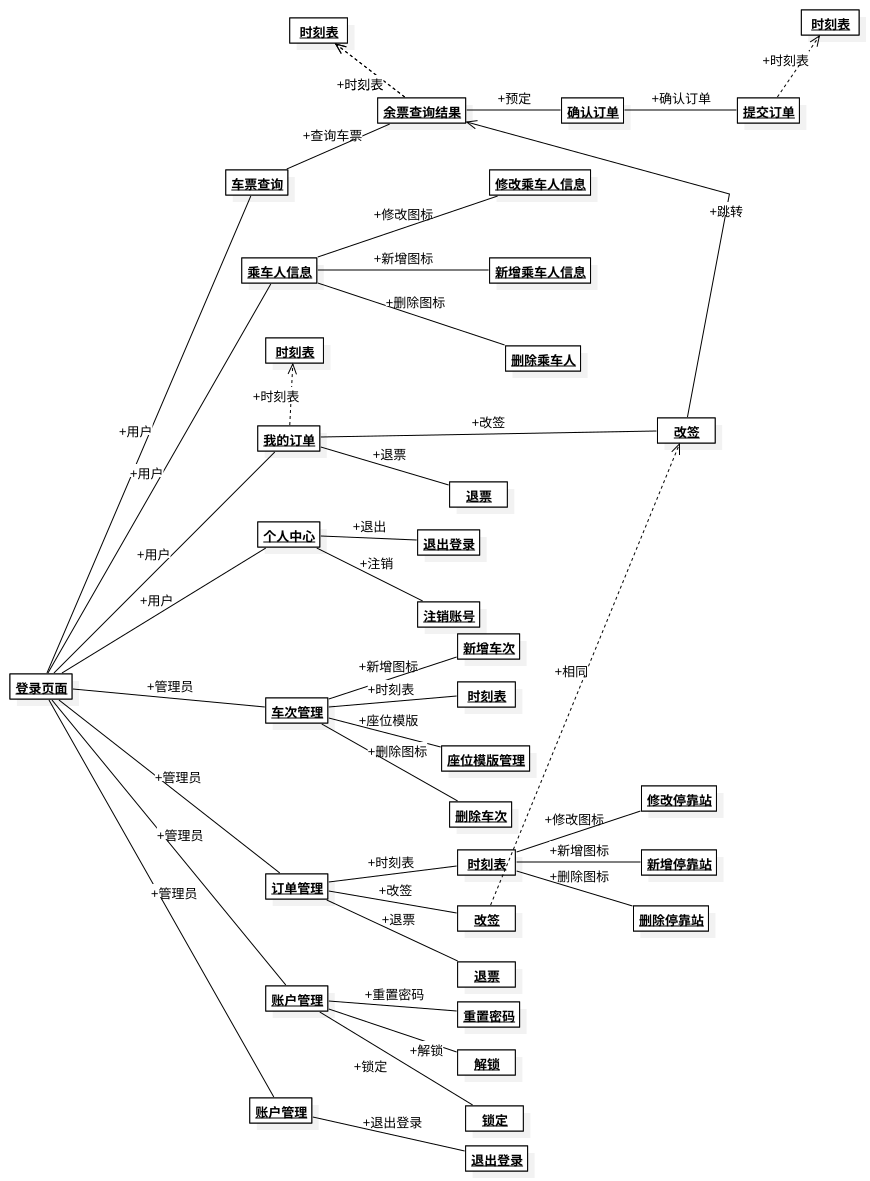
\includegraphics[width=\textwidth]{前端点击流程图.svg}
		\caption{页面跳转逻辑图}
	\end{figure}
	
	\subsection{登录界面}
	登录页 \texttt{Login.qml} 是一个可嵌入的页面，由 \texttt{main.qml} 用 \texttt{Loader} 覆盖在主界面之上。用户可以在“用户登录/管理员登录”之间切换（\texttt{isAdminLogin}），界面会用颜色和字体变化提示当前模式。点击登录后分别调用 \texttt{accountManager.loginUser\_api(...)} 或 \texttt{accountManager.loginAdmin\_api(...)}。登录成功就把 \texttt{SessionState.role} 和 \texttt{SessionState.username} 写进去，再把 \texttt{SessionState.isLoggedIn} 置为 \texttt{true}，随后触发 \texttt{loadStartPage()} 跳到对应的起始页（加一点延时是为了让页面容器先准备好）。
	
	% ====== 插入两张图：用户登录、管理员登录 ======
	\begin{figure}[H]
		\centering
		\begin{subfigure}[t]{0.48\textwidth}
			\centering
			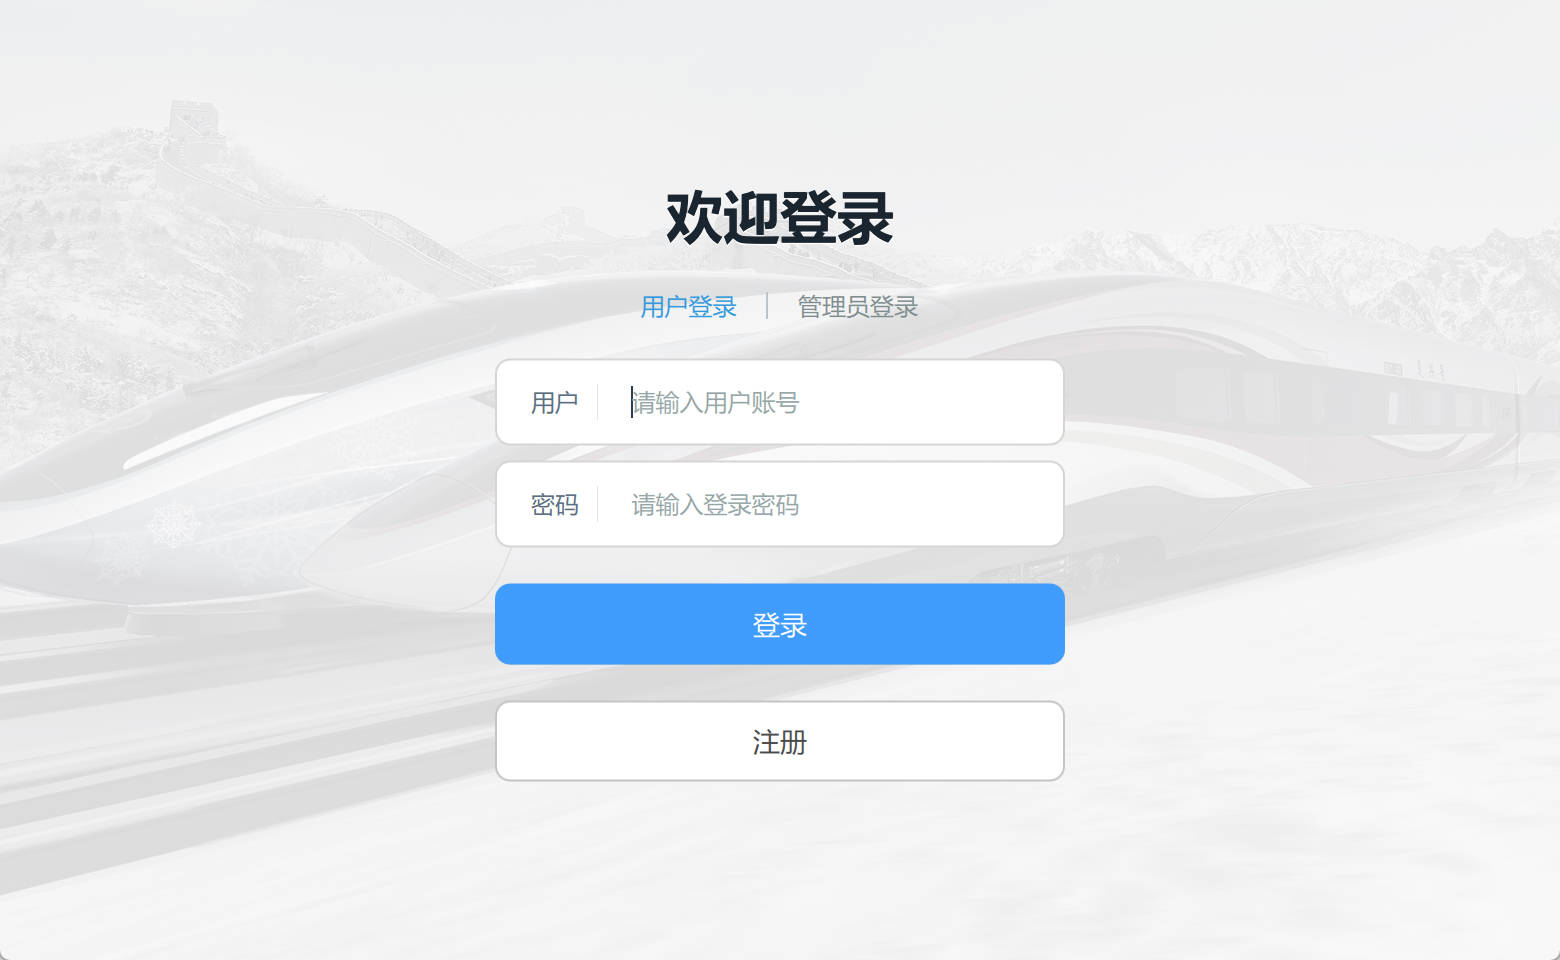
\includegraphics[width=\textwidth]{用户登录.jpg}
			\caption{用户登录}
		\end{subfigure}\hfill
		\begin{subfigure}[t]{0.48\textwidth}
			\centering
			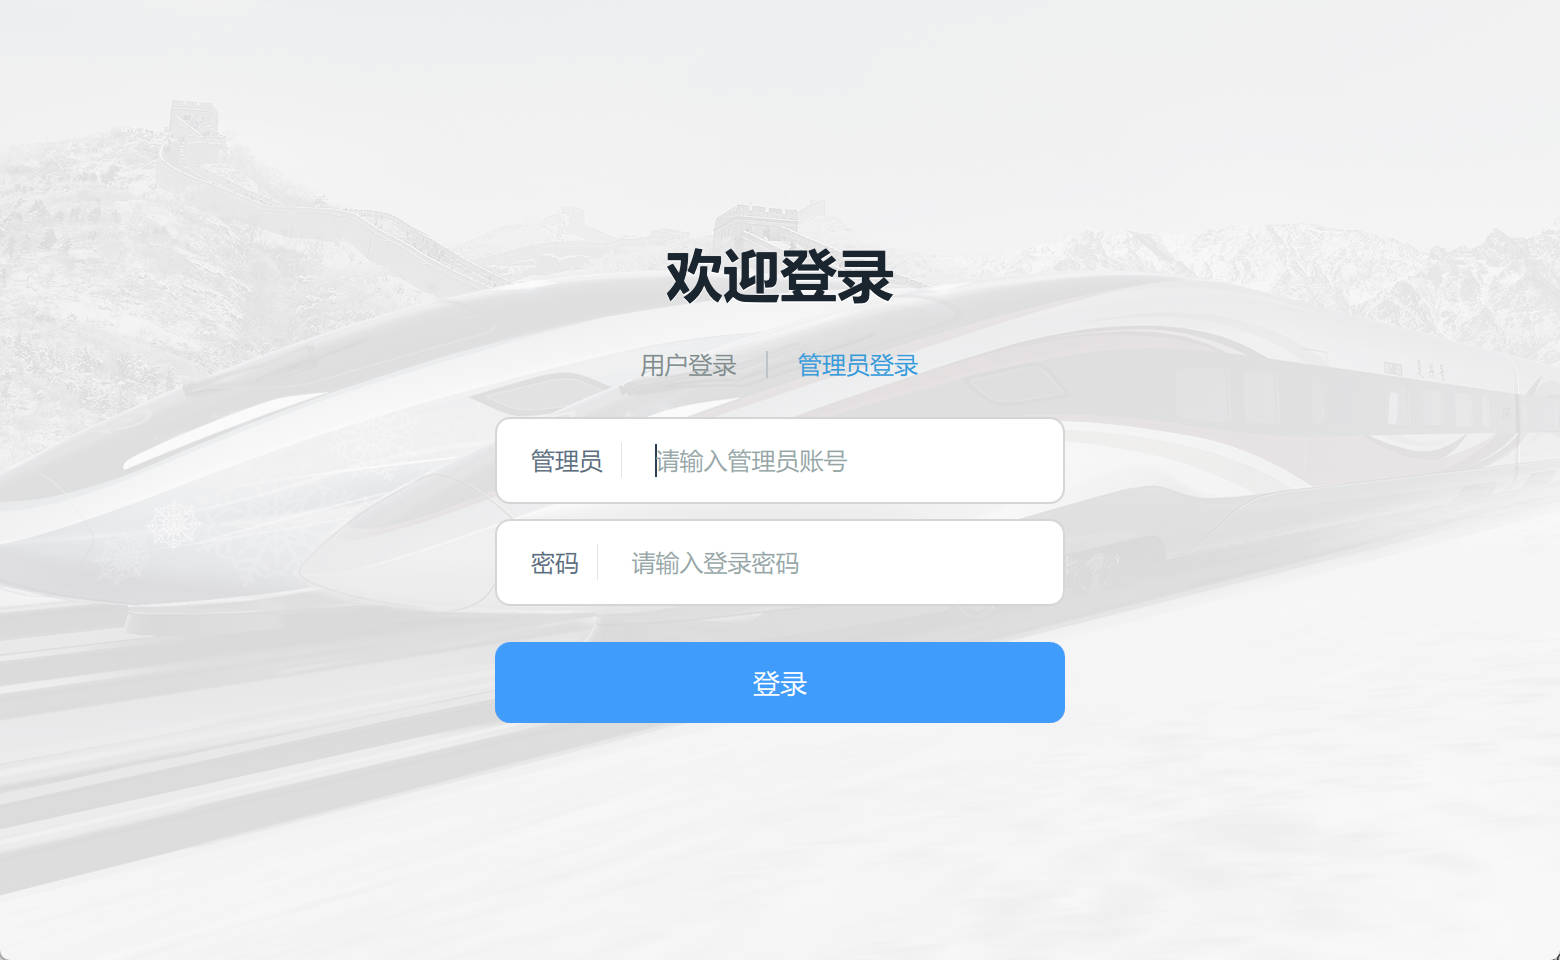
\includegraphics[width=\textwidth]{管理员登录.jpg}
			\caption{管理员登录}
		\end{subfigure}
		\caption{登录界面展示}
	\end{figure}
	
	\subsection{订单流程页面（从查询到提交）}
	整个订票流程从 \texttt{TicketQuery.qml} 开始。页面会先从 \texttt{stationManager.getCitiesName\_api()} 拿到城市列表，用户选择出发地和目的地后点击查询；同时会调用 \texttt{bookingSystem.addQueryHistory\_api(from,to)} 记一条查询历史，方便下次复用。查询结果在 \texttt{TicketQueryResult.qml} 里展示，它用一个独立的 \texttt{Window} 弹出来并设为模态（\texttt{Qt.WindowModal}），这样用户不会在中途跑去点其它页面导致流程断掉。筛选与排序主要在前端对结果列表做处理，减少重复请求；如果是改签模式（\texttt{rescheduleMode=true}），一些容易误操作的交互（比如交换出发/到达）会被禁用，并给出相应的鼠标提示。
	
	选中车次后进入确认窗口 \texttt{OrderConfirm.qml}：这里把“车票信息、乘车人选择、价格展示”集中在一处完成。普通购票会调用 \texttt{bookingSystem.getPassengers\_api(\{...\})}，后端会给出每个乘车人在该时间段是否可用的标记 \texttt{available}；改签场景则调用 \texttt{orderManager.getPassengerForReschedule\_api(...)}，直接加载原订单对应的乘车人并尽量默认选中。界面上不可用的乘车人会提示原因，相关按钮也会自动变灰并禁止点击；总价会随勾选即时更新，给用户一个直观反馈。
	
	最后是提交弹窗 \texttt{SubmitOrderDialog.qml}，采用无边框样式并支持拖动，桌面端体验更自然。点击“提交订单”会调用 \texttt{bookingSystem.createOrder\_api(\{...\})} 完成落单；改签时管理员端不会强行传 \texttt{username}，由后端从待改签订单反查归属，减少传参不一致带来的问题。提交结束会弹出提示，并通过信号通知上层刷新列表或关闭窗口。
	
	% ====== 插入四张图：车票查询、车票选择、确认订单、提交订单 ======
	\begin{figure}[H]
		\centering
		\begin{subfigure}[t]{0.48\textwidth}
			\centering
			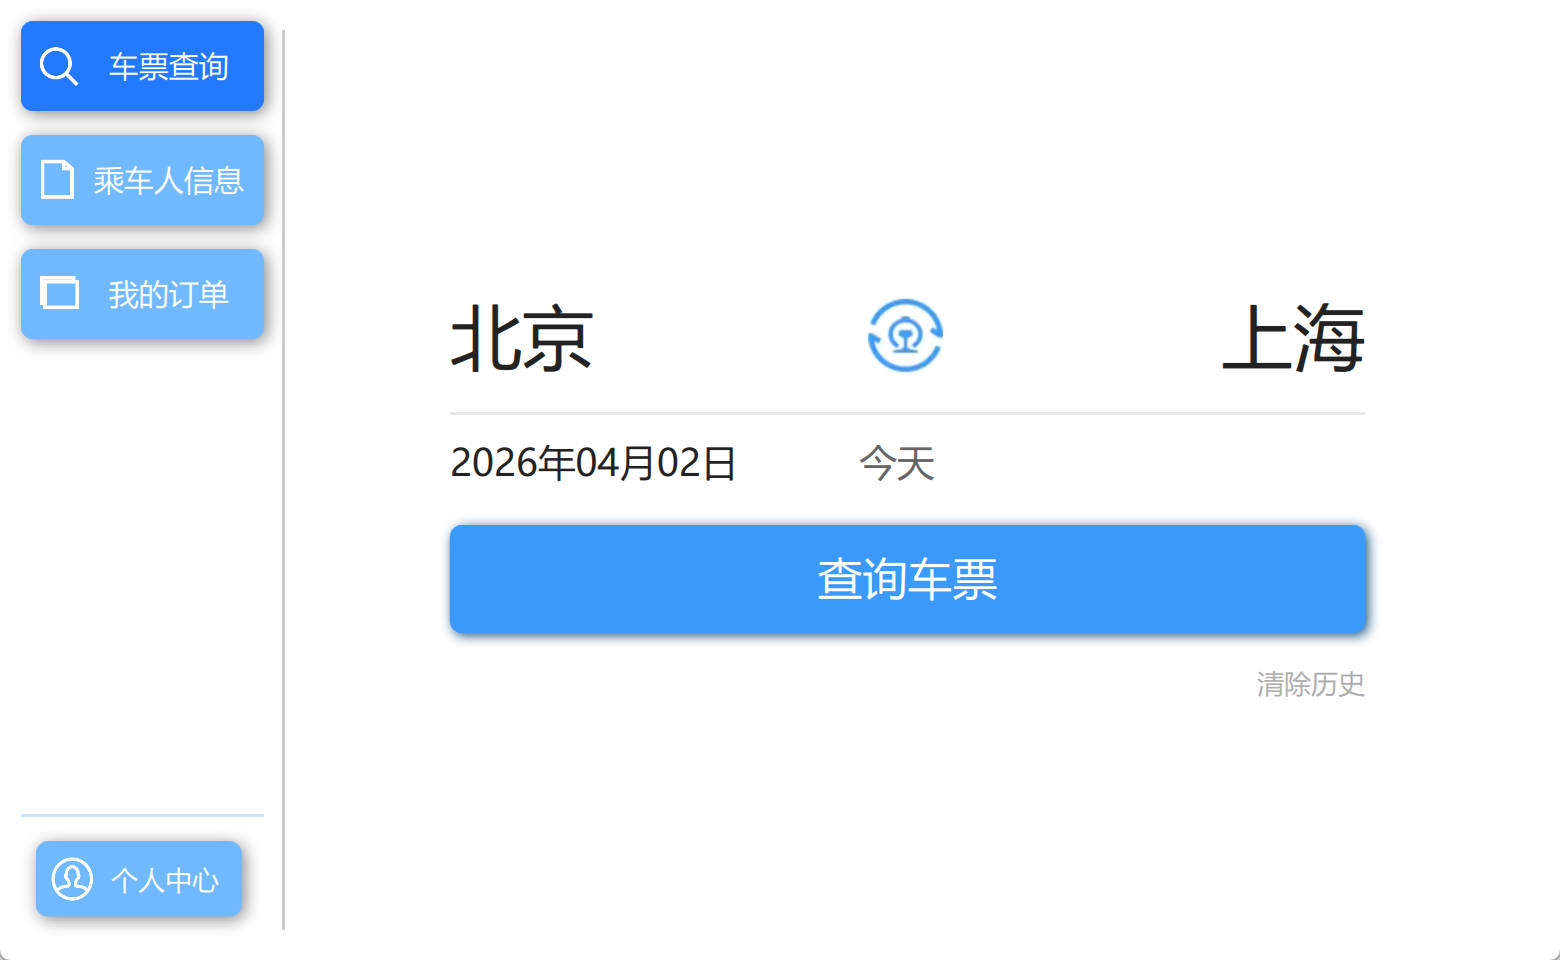
\includegraphics[width=\textwidth]{车票查询.jpg}
			\caption{车票查询}
		\end{subfigure}\hfill
		\begin{subfigure}[t]{0.48\textwidth}
			\centering
			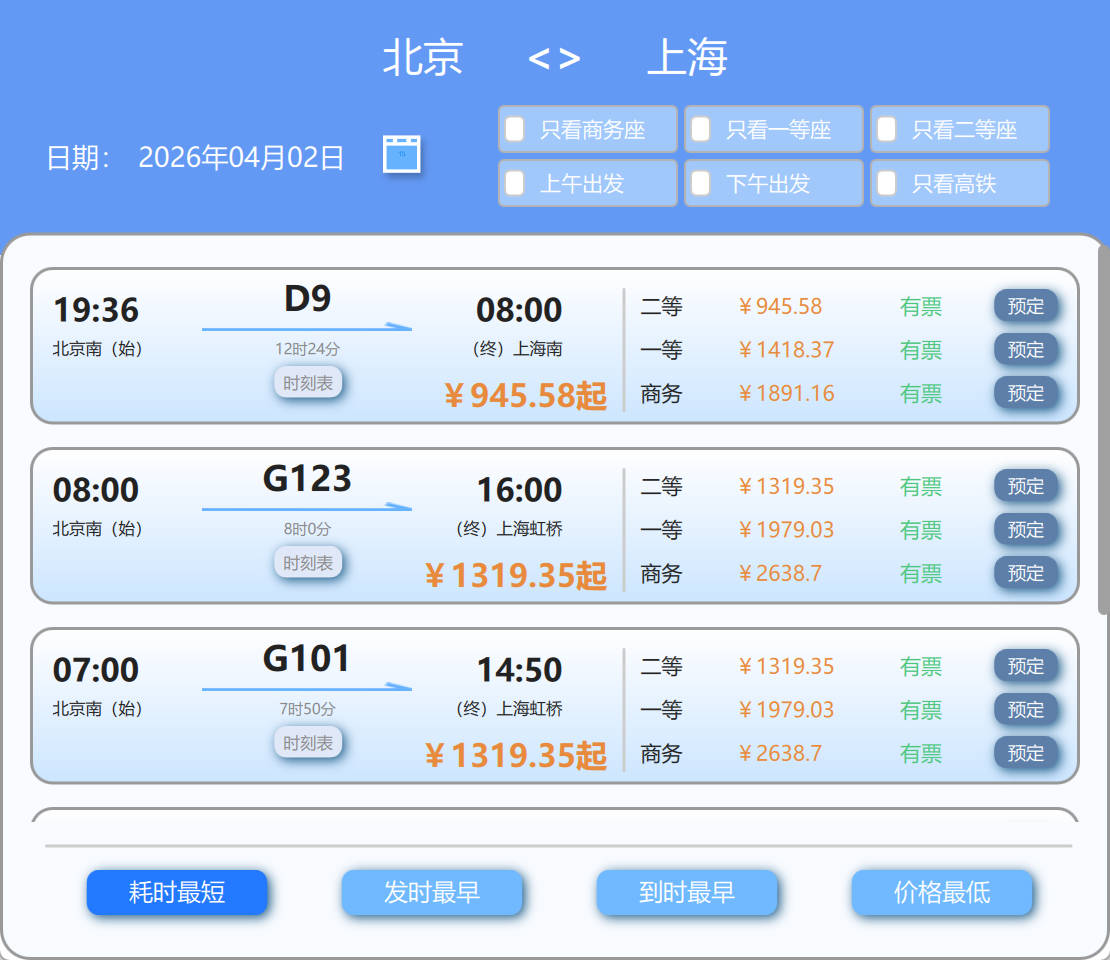
\includegraphics[width=\textwidth]{车票选择.jpg}
			\caption{车票选择}
		\end{subfigure}
		
		\vspace{0.4cm}
		
		\begin{subfigure}[t]{0.48\textwidth}
			\centering
			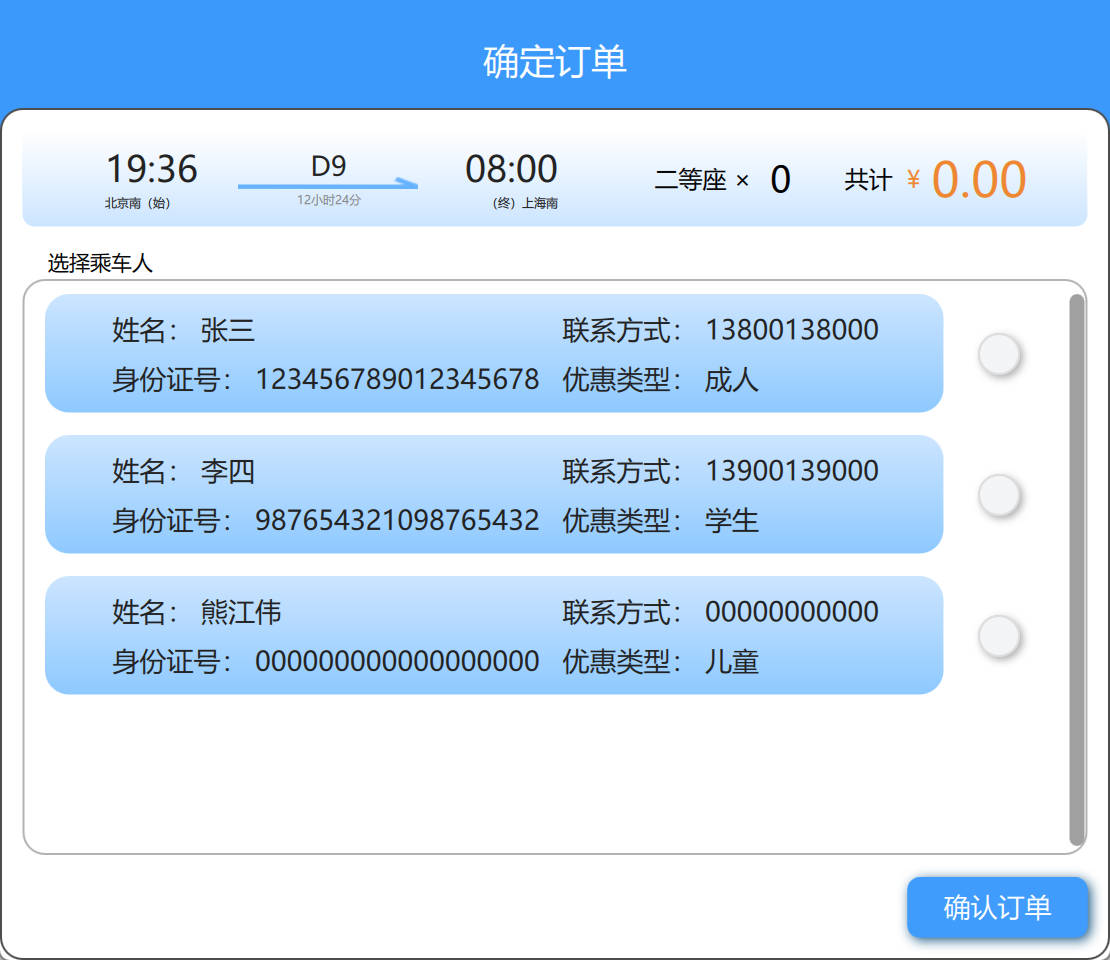
\includegraphics[width=\textwidth]{确定订单.jpg}
			\caption{确定订单}
		\end{subfigure}\hfill
		\begin{subfigure}[t]{0.48\textwidth}
			\centering
			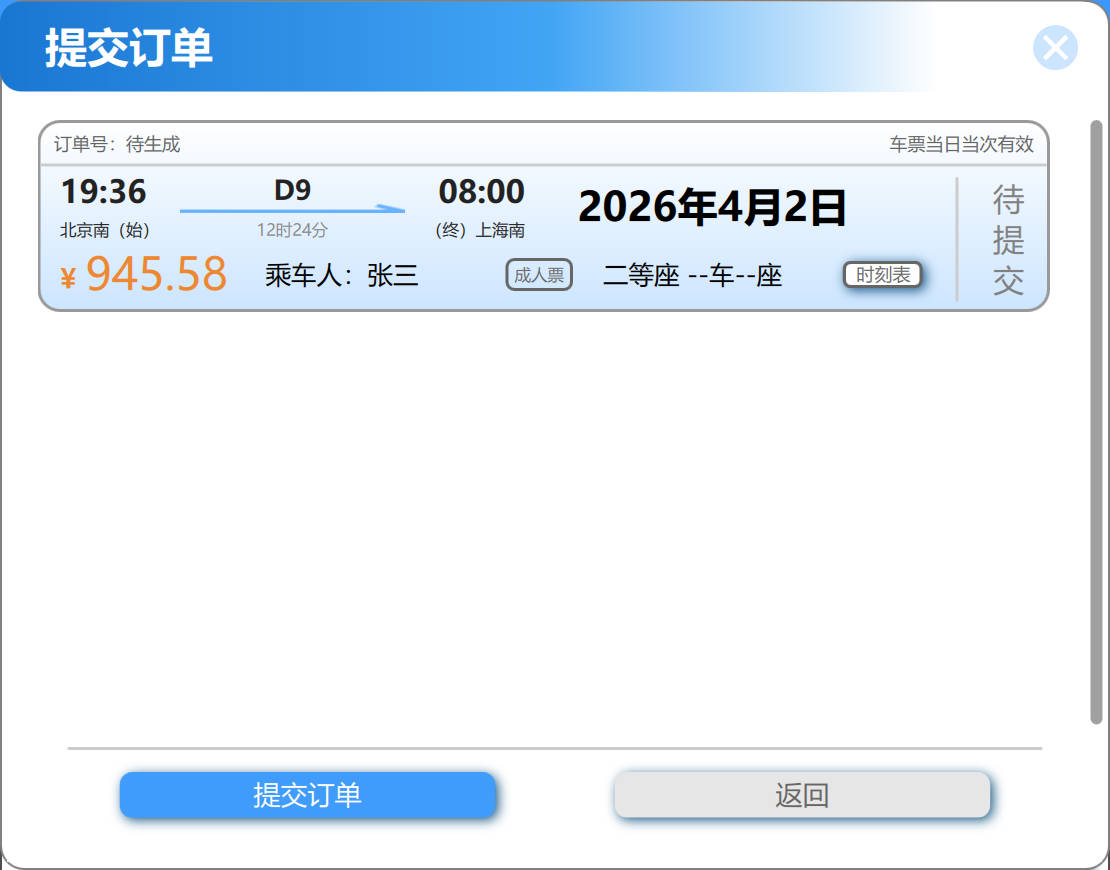
\includegraphics[width=\textwidth]{提交订单.jpg}
			\caption{提交订单}
		\end{subfigure}
		\caption{订单流程页面展示}
	\end{figure}
	
	\subsection{订单管理界面（用户/管理员）}
	用户端的“我的订单”在 \texttt{MyOrders.qml} 中实现，用 \texttt{ListView} 配合 \texttt{OrderCard} 以卡片形式展示，滚动条样式统一。订单卡片提供改签与退票等操作，并按状态做限制：只有 \texttt{status=="待乘坐"} 的订单才允许改签；退票会先弹出确认框，避免误点。页面还提供多条件搜索（订单号、车次、日期、乘车人、站点），订单多的时候更好找。
	
	管理员端 \texttt{OrderManagement.qml} 的界面结构与用户端基本一致，复用同一套卡片与搜索方式，主要区别在于数据是全量订单；操作同样有状态限制和确认弹窗，保证处理逻辑一致。
	
	% ====== 插入两张图：用户订单管理、管理员订单管理 ======
	\begin{figure}[H]
		\centering
		\begin{subfigure}[t]{0.48\textwidth}
			\centering
			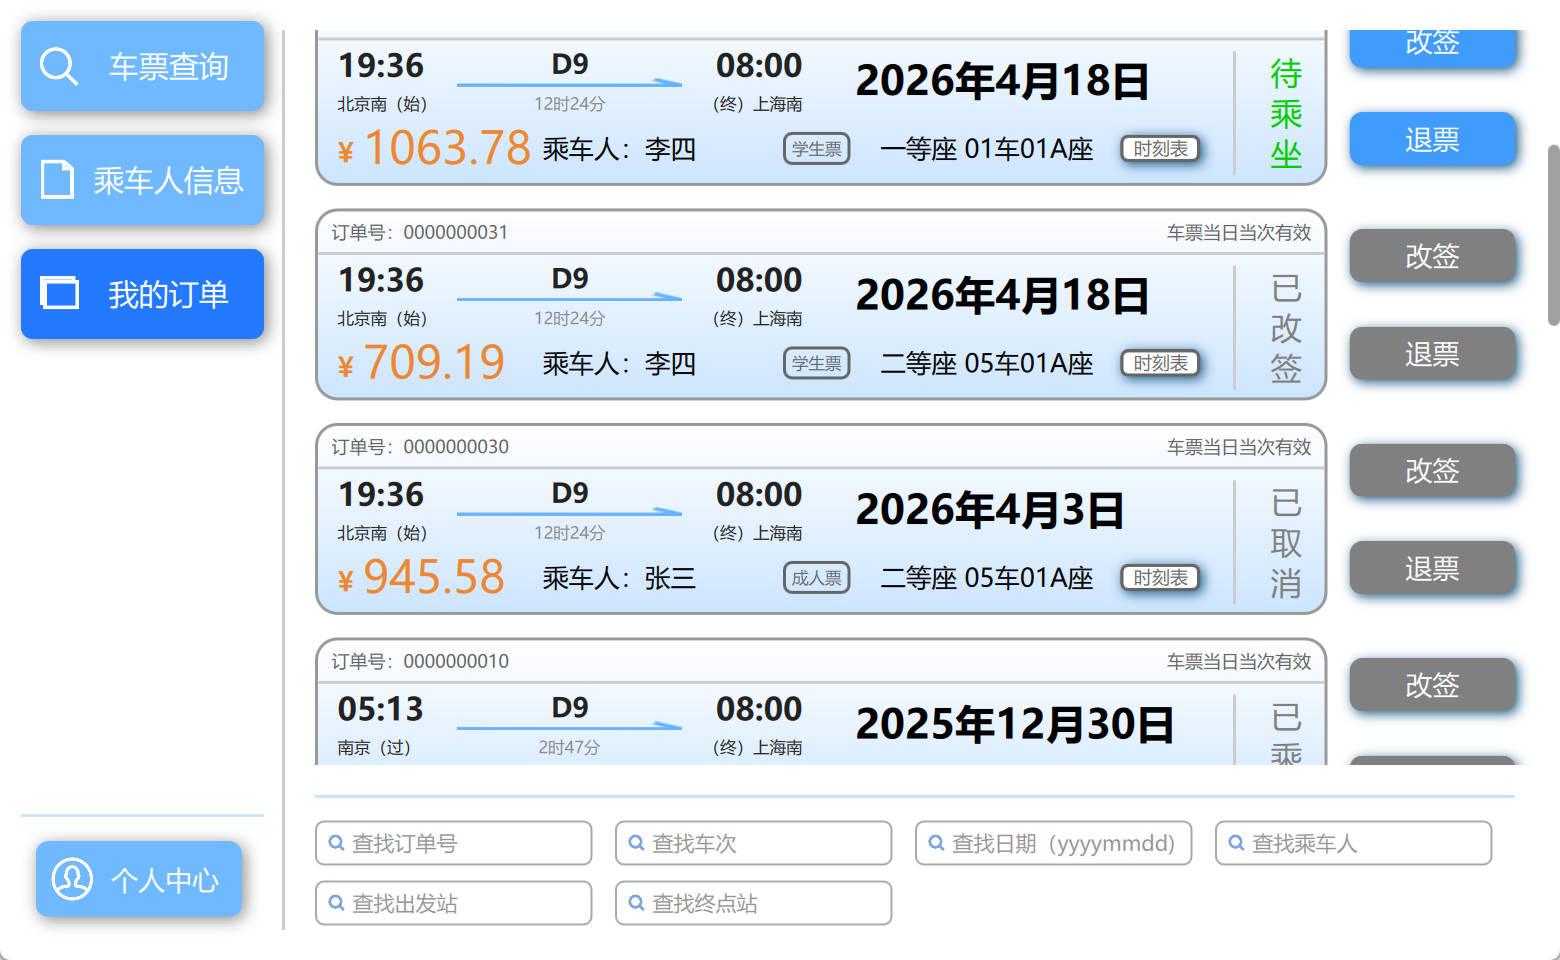
\includegraphics[width=\textwidth]{用户订单管理.jpg}
			\caption{用户订单管理}
		\end{subfigure}\hfill
		\begin{subfigure}[t]{0.48\textwidth}
			\centering
			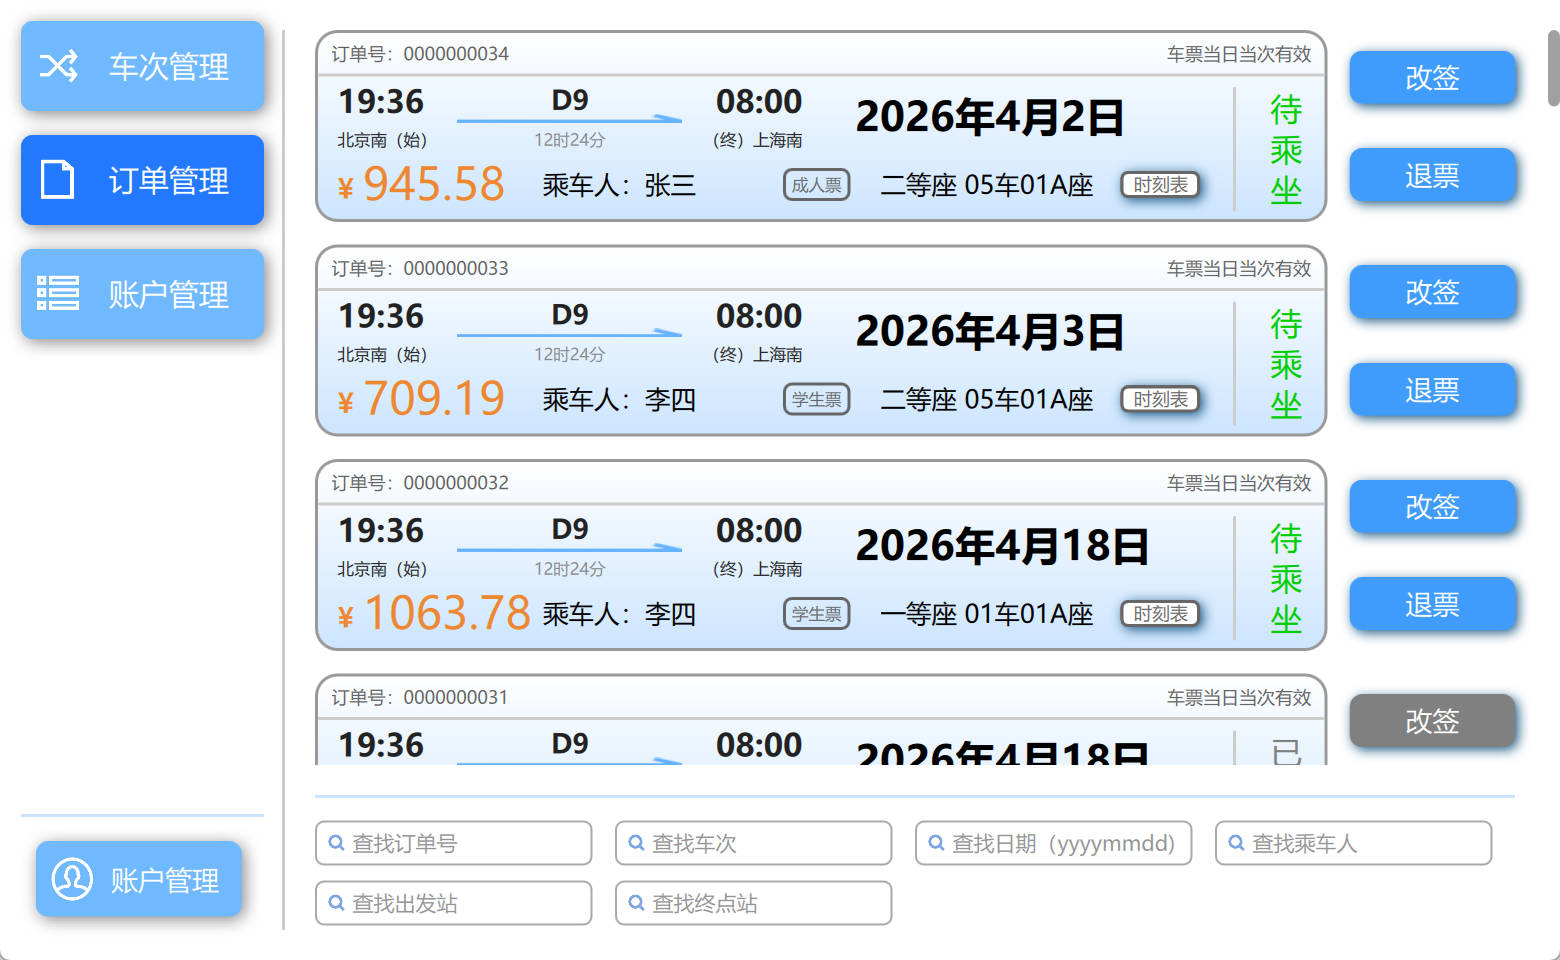
\includegraphics[width=\textwidth]{管理员订单管理.jpg}
			\caption{管理员订单管理}
		\end{subfigure}
		\caption{订单管理界面展示}
	\end{figure}
	
	\subsection{管理员后台页面}
	车次管理页 \texttt{TrainManagement.qml} 用 \texttt{TrainCard} 展示车次列表，并提供时刻表、座位模板与删除等入口。删除前会先做可编辑性检查（例如 \texttt{isTrainEditable(...)}），如果车次存在风险（如仍有关联的待乘坐订单）则直接阻止删除并提示原因。编辑相关功能采用 \texttt{Loader} 按需加载弹窗（时刻表管理、座位模板编辑等），主页面保持简洁，也能减少卡顿。
	
	账户管理页 \texttt{UserManagement.qml} 用 \texttt{AccountCard} 展示账号信息，提供重置密码、锁定、解锁等操作。危险操作统一要二次确认，并且做了基本的防呆：例如管理员不能锁定自己（当 \texttt{SessionState.username == modelData.username} 时直接拦截并提示）。
	
	% ====== 插入两张图：车次管理、账户管理 ======
	\begin{figure}[H]
		\centering
		\begin{subfigure}[t]{0.48\textwidth}
			\centering
			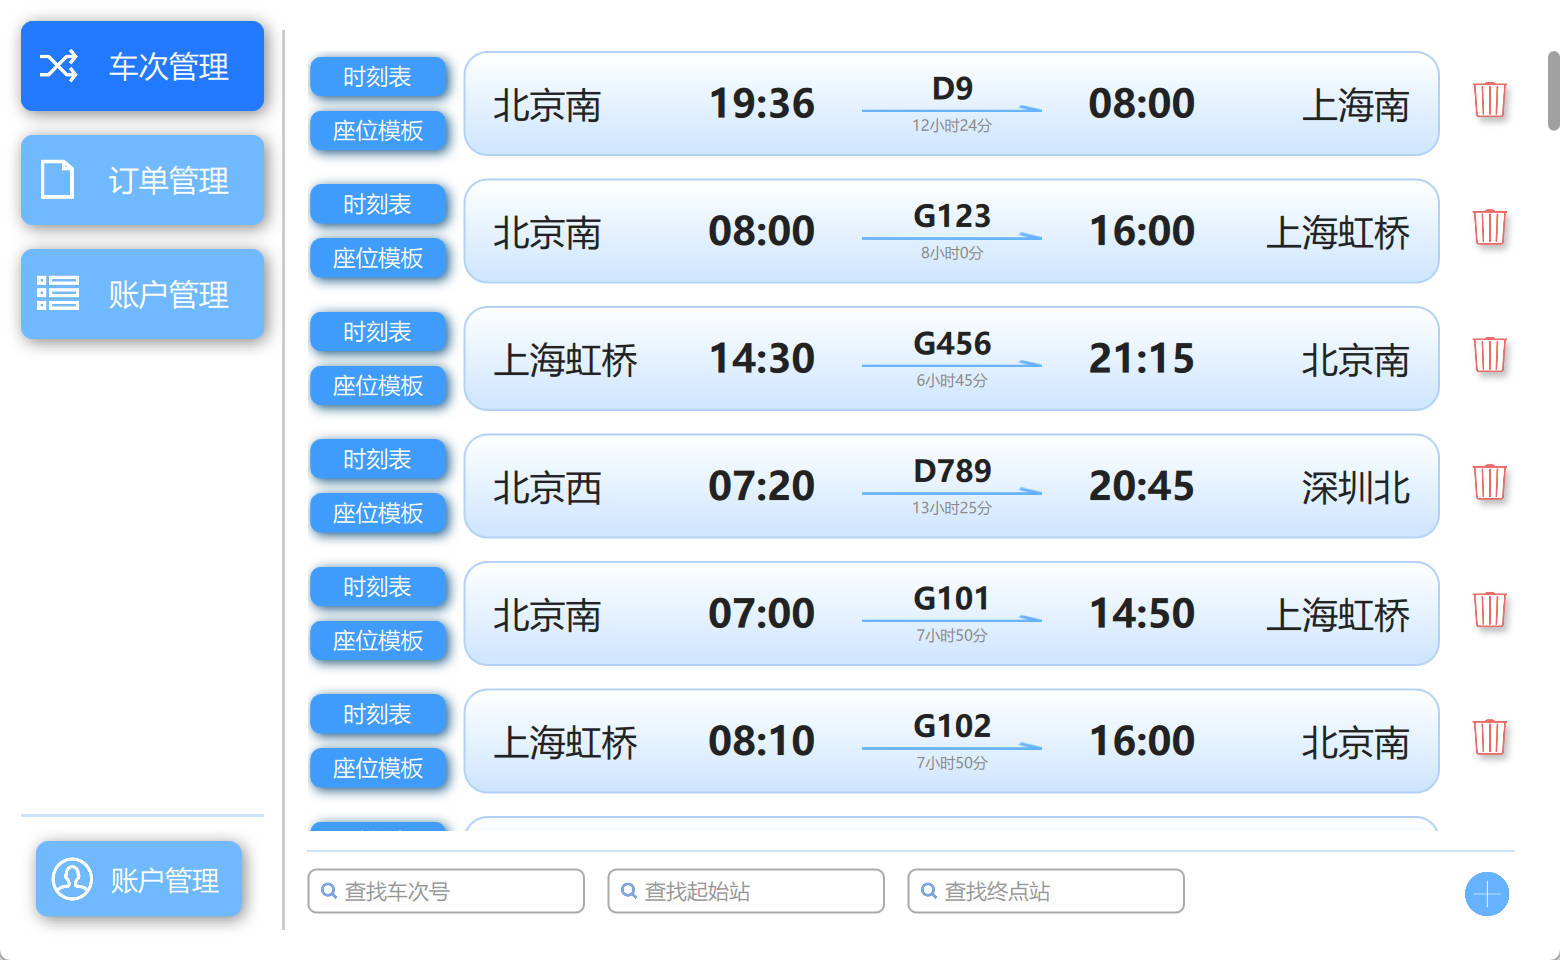
\includegraphics[width=\textwidth]{车次管理.jpg}
			\caption{车次管理}
		\end{subfigure}\hfill
		\begin{subfigure}[t]{0.48\textwidth}
			\centering
			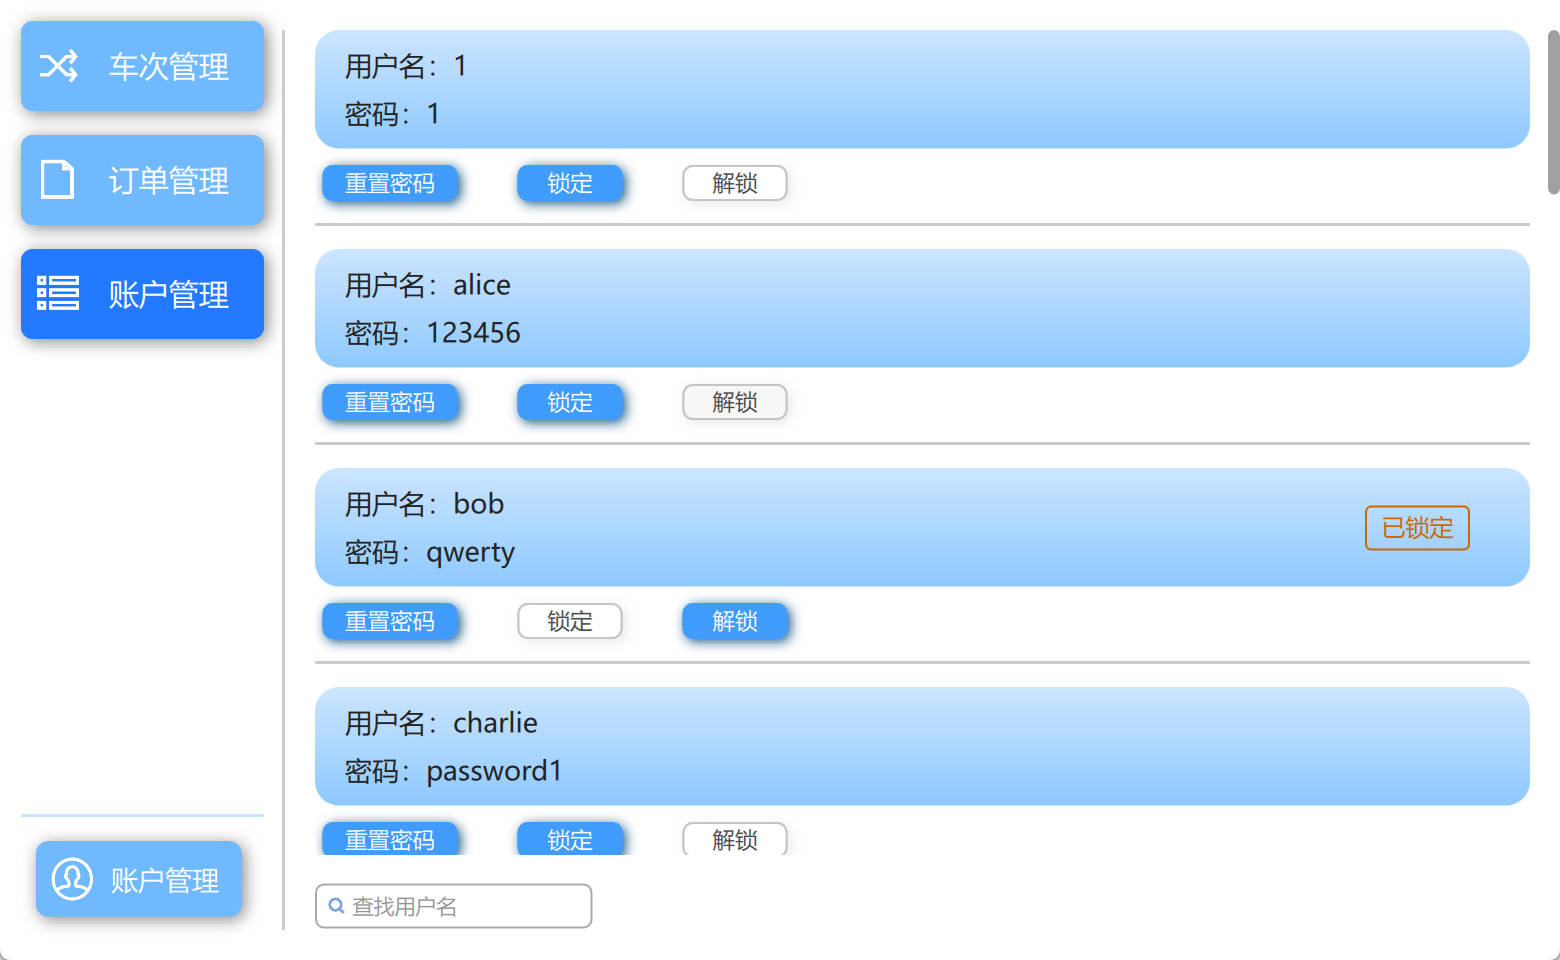
\includegraphics[width=\textwidth]{账户管理.jpg}
			\caption{账户管理}
		\end{subfigure}
		\caption{管理员后台页面展示}
	\end{figure}
	
	\subsection{页面组织与导航（StackView + Loader）}
	主内容区由 \texttt{StackView} 承载。侧边栏点击菜单后会清空当前栈并进入目标页面（\texttt{stackView.clear(); stackView.push(pageUrl, \{...\})}），同时在 \texttt{onCurrentItemChanged} 中同步菜单选中态，保证“当前页”��“菜单高亮”一致。登录页则用 \texttt{Loader} 覆盖主界面：未登录时把主内容遮住，登录成功后再移除覆盖层，避免出现页面还没准备好就被误操作的情况。
	
\end{document}